\documentclass[12pt,a4paper]{article}
\usepackage{amsmath}
\usepackage{amsfonts}
\usepackage{amssymb}
\usepackage{graphicx}
\usepackage{secdot}
\usepackage{multirow}
\usepackage[left=2cm,right=2cm,top=2cm,bottom=2cm]{geometry}

\title{{Experiment - 5\\ \textbf{Pressure distribution over a circular cylinder}}}
\author{Arka Pramanick, AE21B007\\ Department of Aerospace Engineering\\ IIT Madras\\[3ex] Instructor:\\ \large Professor Dr. R. Sriram}

\date{14 March, 2023}


\begin{document}
\maketitle

\hline

\section{Aim :}
\begin{itemize}
    \item Analysing pressure distribution and flow behaviour through a circular cylinder.
    \item Comparison of Theoretical and Experimental Coefficient of pressure at different points on circular cylinder.
\end{itemize}


\section{Apparatus :}
Required apparatus for performing this experiment are:
\begin{itemize}
    \item Manometer
    \item C15-10 Armfield tunnel
    \item Pitot-static Probe
    \item Fan
\end{itemize}

\begin{figure}[!ht]
	\begin{center}
		\framebox{
			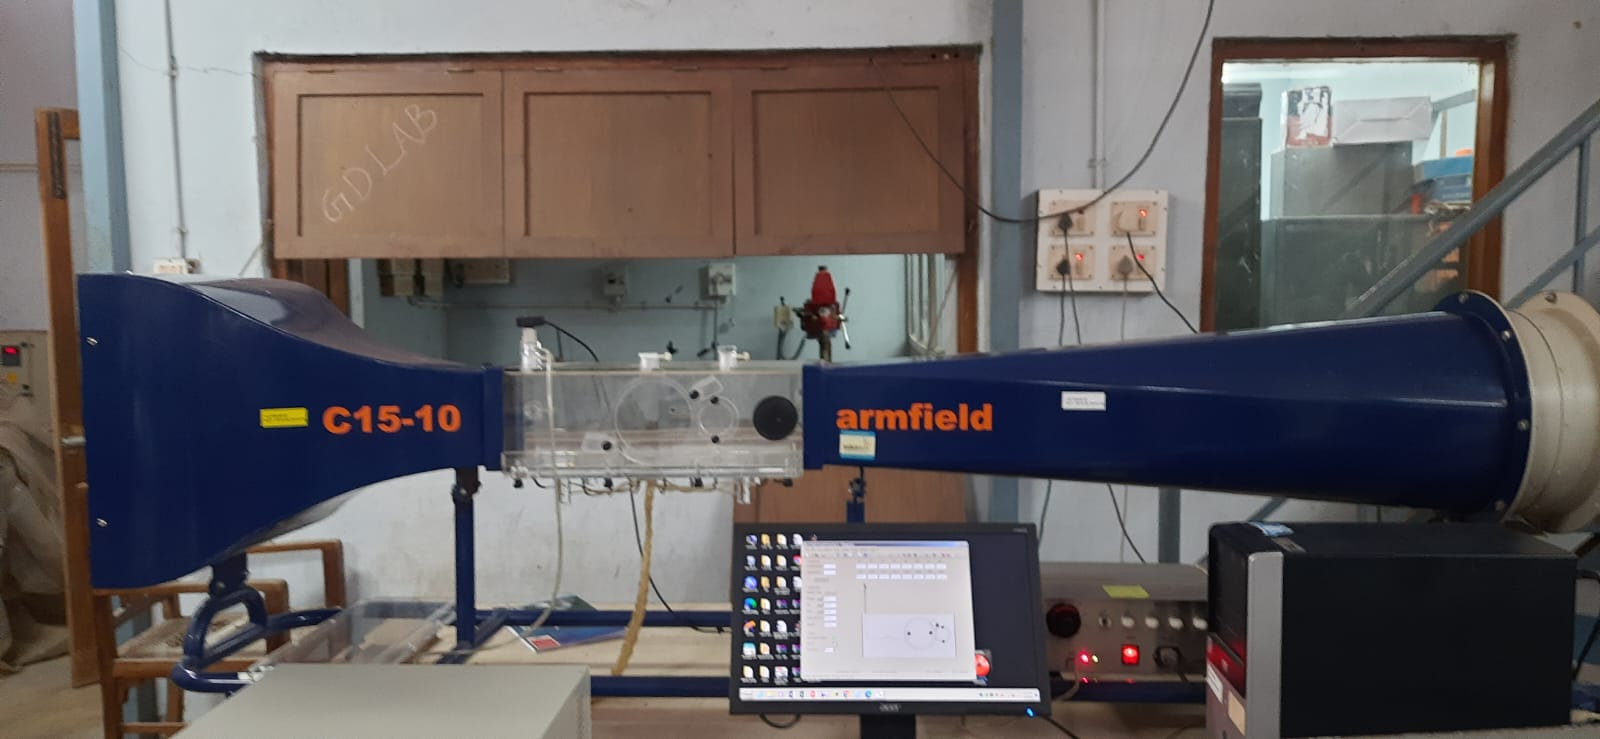
\includegraphics[scale=0.2]{wind tunnel.jpg}
		}
	\end{center}
	\caption{C15-10 Armfield}
\end{figure}


\newpage
\section{Theory :}

Considering a circular cylinder immersed in a uniform flow,the streamlines are shown as :
\begin{figure}[!ht]
	\begin{center}
		\framebox{
			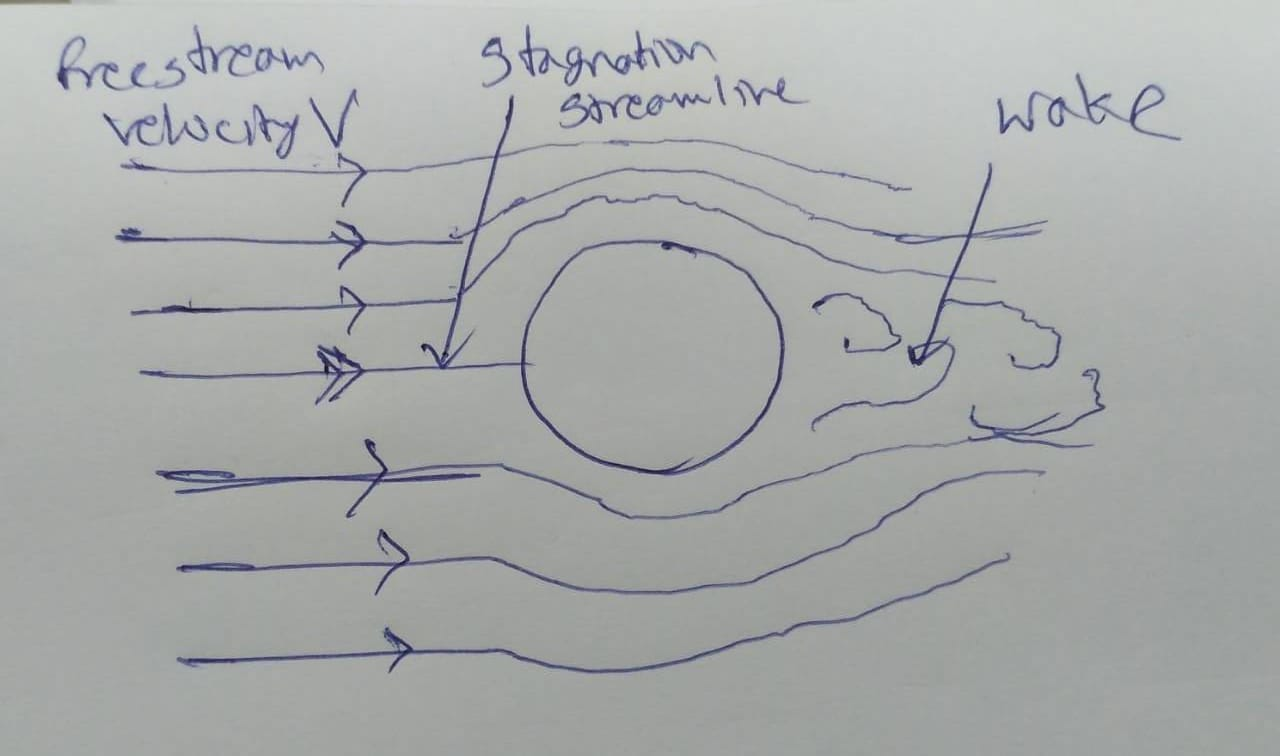
\includegraphics[scale=0.2]{exp 5 cylinder.jpg}
		}
	\end{center}
	\caption{Streamlines of a flow through a circular Cylinder}
\end{figure}



At stagnation point ($P = P_0 $),no lifting flow or drag exists.Here velocity becomes maximum and pressure becomes minimum.
The pressure exerted by the fluid on the on the front half of the cylinder is higher than pressure exerted on rear half.If the difference of this pressure is multiplied by projected area Drag Force is obtained.Unequal pressure distribution is observed across the cylindrical surface. 



For flow around a circular cylinder can be considered as a uniform flow with a doublet.
Therefore, $$ W(z) = U_{\infty} Z + \frac{K}{Z} $$ 
Stream function($\Psi$) = $U_{\infty} r sin\theta -\frac{K sin\theta}{r}$ \\
Velocity potential ($\phi$) = $U_{\infty} r cos\theta + \frac{K cos\theta}{r}$ \\


Velocity components are given by,
$$V_r = \frac{1}{r} \frac{\delta \psi}{\delta \theta} = cos\theta(U_{\infty}- \frac{K}{r^2})$$
$$V_{\theta} = -\frac{\delta \psi}{\delta r} = -sin\theta (U_{\infty} + \frac{K}{r^2}) $$
Velocity components on the surface of cylinder(r = a) are:\\
 $V_r_s = 0 , V_{\theta}_s = -2U_{\infty} sin\theta $ \\

For $\theta $ = 0° and 180° , $V_r_s = V_{\theta}_s = 0 $ \\
These are the points denoting stagnation point. The velocity decreases from a value of $2U_{\infty}$ at $\theta = 90 ^{\circ}$ to $U_{\infty}$ on moving away in a normal direction.

Applying Bernoulli equation, \\
$$ P_{\infty} + \frac{\rho U_{\infty}^{2}}{2} = P_s +  \frac{\rho V_{\theta}_s^{2}}{2} $$ 
Substituting for $V_{\theta}_s = -2U_{\infty} sin{\theta}$

$$ C_p = \frac{P_s - P_{\infty}}{q_{\infty}} $$
$$C_p = 1- 4 {\sin^2{\theta}} $$
In the graph of $C_p$ vs $\theta$, the region to the right of the center-line separation of flow is observed as viscous force dominates here.\\



Due to the pressure differential, the flowing fluid exerts \textbf{Drag skin friction} between the fluid and the cylinder, causing drag. \\
\underline{Coefficient of Drag ($C_d$)} is calculated by :
$$ C_d = \frac{D/l}{(1/2)\rho v^2 S} $$ \\
S = 2$\pi$ R \\




   




\section{Procedure :}
\begin{enumerate}
    \item In wind tunnel test section is set.
    \item Pitot-static probe is connected to manometer.
    \item Fan speed is fixed.
    \item Required readings are taken.
\end{enumerate}






\section{Observation :}



\subsection{For Velocity = 10.2 m/s : } 

\begin{table}[ht]
\centering
\caption{\textbf{Theoretical and Experimental $C_p$ at different points on the surface of a cylinder for velocity 10.2 m/s}}
\vspace{2mm}
\begin{flushleft}
\begin{tabular}{|c{5 mm}|c{15 mm}|c{15 mm}|c{15 mm}|c{15 mm}|} 
 \hline
Points & Distance of Ports from stz & auge Pressure(in mm of water) & Theoretical $C_p$ & Experimental $C_p$\\ [0.01ex] 
 \hline
$P_1$ & 0 & 0.3  & 1 & -0.044 \\ 
 \hline
$P_2$ & 20 & 2.6 & 0.532 & -0.379  \\
 \hline
$P_3$ & 40 & 9.9 & -0.653 & -1.442  \\
 \hline
$P_4$ & 60 & 14.4 & -2 & -2.098  \\
 \hline
$P_5$ & 80 & 13.7 & -2.879 & -1.996  \\
 \hline
$P_6$ & 100 & 13.2 & -2.879 & -1.923 \\ 
 \hline
$P_7$ & 120 & 13.5 & -2 & -1.967 \\ 
 \hline
$P_8$ & 140 & 12.0 & -0.653 & -1.748\\
 \hline
$P_9$ & 160 & 14 & 0.532 & -2.040\\
 \hline
$P_{10}$ & 180 & 0.3 & 1 & -0.044 \\ 
 \hline 


\end{tabular}
\end{flushleft}
\end{table}

\begin{figure}[!ht]
	\begin{center}
		\framebox{
			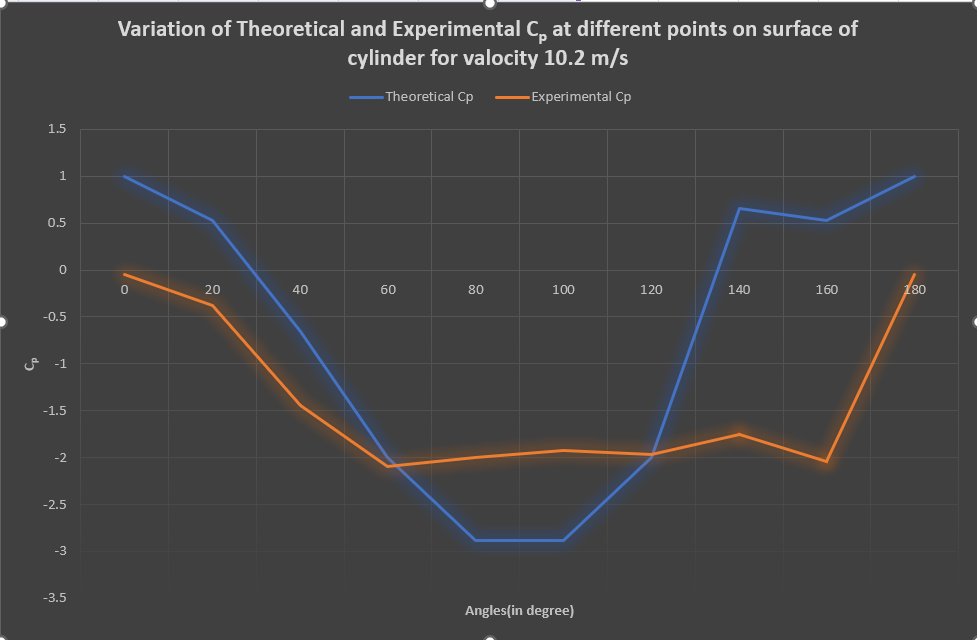
\includegraphics[scale=0.6]{ex 5.1.png}
		}
	\end{center}
	\caption{Variation of theoretical and experimental $C_p$ with Angles}
\end{figure}


\newpage
\subsection{For Velocity = 8.1 m/s : }
\begin{table}[ht]
\centering
\caption{\textbf{Theoretical and Experimental $C_p$ at different points on the surface of a cylinder for velocity 8.1 m/s}}
\vspace{2mm}
\begin{flushleft}
\begin{tabular}{|c|c|c|c|c|} 
 \hline
Points & Angle(in degrees) & Gauge Pressure(in mm of water) & Theoretical $C_p$ & Experimental $C_p$\\ [0.1ex] 
 \hline
$P_1$ & 0 & 0.3  & 1 & -0.069 \\ 
 \hline
$P_2$ & 20 & 1.9 & 0.532 & -0.439  \\
 \hline
$P_3$ & 40 & 4.4 & -0.653 & -1.017  \\
 \hline
 $P_4$ & 60 & 8.3 & -2 & -1.918  \\
 \hline
$P_5$ & 80 & 8.2 & -2.879 & -1.895  \\
 \hline
$P_6$ & 100 & 8 & -2.879 & -1.848 \\ 
 \hline
$P_7$ & 120 & 8.1 & -2 & -1.871 \\ 
 \hline
$P_8$ & 140 & 7.3 & -0.653 & -1.687\\
 \hline
$P_9$ & 160 & 8.2 & 0.532 & -1.895\\
 \hline
$P_{10}$ & 180 & 4.4 & 1 & -1.017 \\ 
 \hline 

\end{tabular}
\end{flushleft}
\end{table}

\begin{figure}[!ht]
	\begin{center}
		\framebox{
			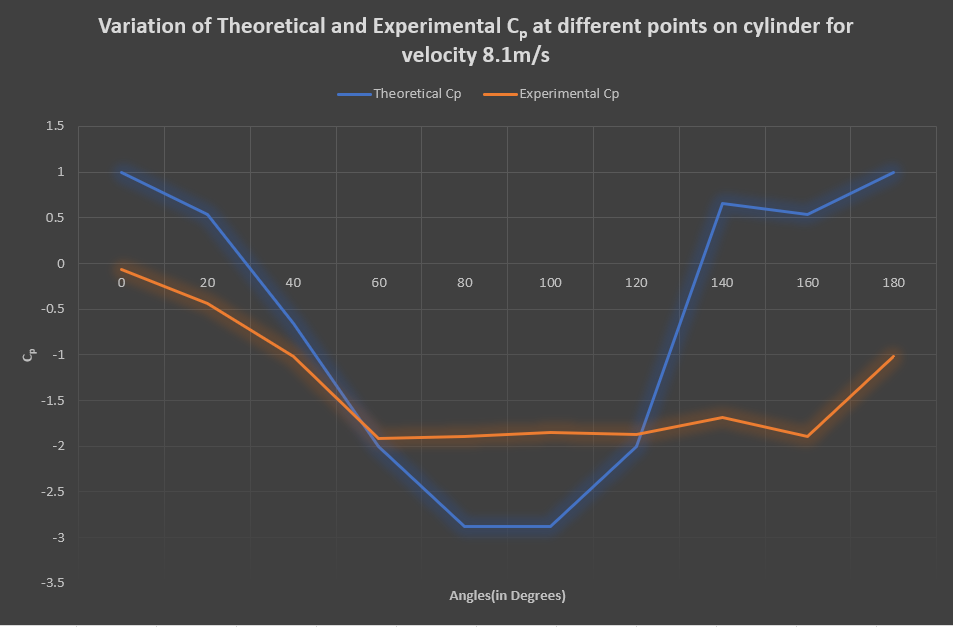
\includegraphics[scale=0.6]{ex5.2.png}
		}
	\end{center}
	\caption{Variation of theoretical and experimental $C_p$ with Angles}
\end{figure}



\newpage


\subsection{For Velocity = 14.3 m/s}
\begin{table}[ht]
\centering
\caption{\textbf{Theoretical and Experimental $C_p$ at different points on the surface of a cylinder for velocity 14.3 m/s}}
\vspace{2mm}
\begin{flushleft}
\begin{tabular}{|c|c|c|c|c|} 
 \hline
Points & Angle(in degrees) & Gauge Pressure(in mm of water) & Theoretical $C_p$ & Experimental $C_p$\\ [0.1ex] 
 \hline
$P_1$ & 0 & 0.6  & 1 & -0.044 \\ 
 \hline
$P_2$ & 20 & 5 & 0.532 & -0.371  \\
 \hline
$P_3$ & 40 & 12.9 & -0.653 & -0.956  \\
 \hline
$P_4$ & 60 & 20.3 & -2 & -1.505  \\
 \hline
$P_5$ & 80 & 19.5 & -2.879 & -1.446  \\
 \hline
$P_6$ & 100 & 19.1 & -2.879 & -1.416 \\ 
 \hline
$P_7$ & 120 & 19.4 & -2 & -1.438 \\ 
 \hline
$P_8$ & 140 & 17.3 & -0.653 & -1.282\\
 \hline
$P_9$ & 160 & 20.1 & -0.532 & -1.490\\
 \hline
$P_{10}$ & 180 & 0.3 & 1 & -0.022 \\ 
 \hline 

\end{tabular}
\end{flushleft}
\end{table}




\begin{figure}[!ht]
	\begin{center}
		\framebox{
			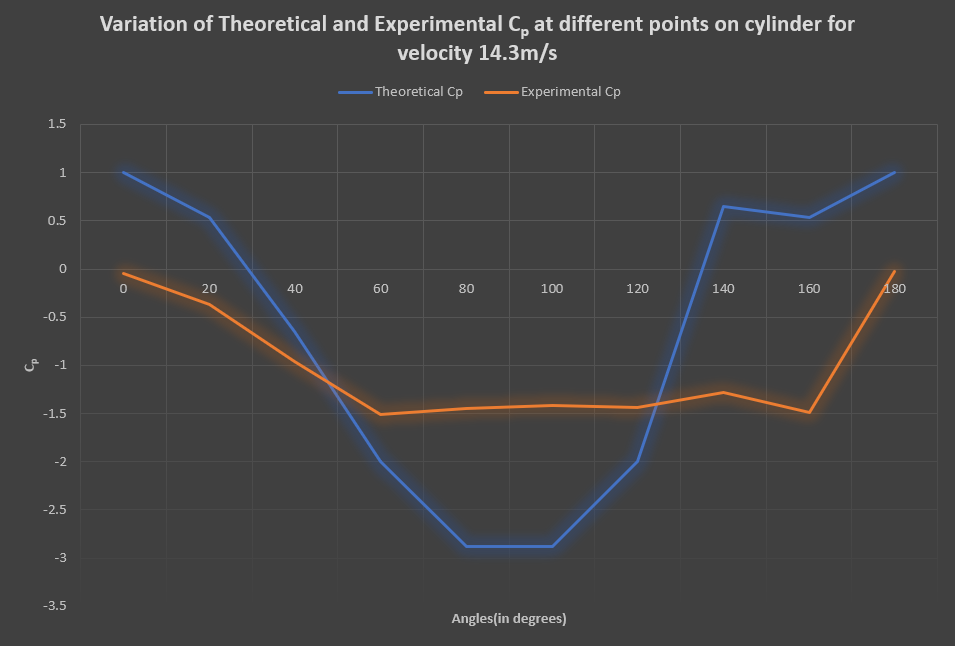
\includegraphics[scale=0.6]{ex5.3.png}
		}
	\end{center}
	\caption{Variation of theoretical and experimental $C_p$ with Angles}
\end{figure}

\newpage

\textbf{Drag vs Velocity : } 



\begin{table}[ht]
\centering
\caption{\textbf{Variation of Drag with Velocity}}
\vspace{2mm}

\begin{tabular}{|c|c|c|c|c|} 
 \hline
Sl No. & Velocity & Drag($\theta = 0^{\circ}$ to $\theta = 180^{\circ}$ & Coeff of Drag($C_d$) \\ [0.1ex] 
 \hline \hline
1 & 8.1 & 0.54 & 0.135   \\ 
 \hline
2 & 10.2 & 1.24 & 0.196  \\
 \hline
3 & 12 & 1.82 & 0.207   \\
 \hline
4 & 14.3 & 2.63 & 0.211   \\
 \hline
5 & 16 & 3.43 & 0.220  \\
 \hline
6 & 18 & 4.25 & 0.215 \\ 
 \hline


\end{tabular}
\end{table}


\begin{figure}[!ht]
	\begin{center}
		\framebox{
			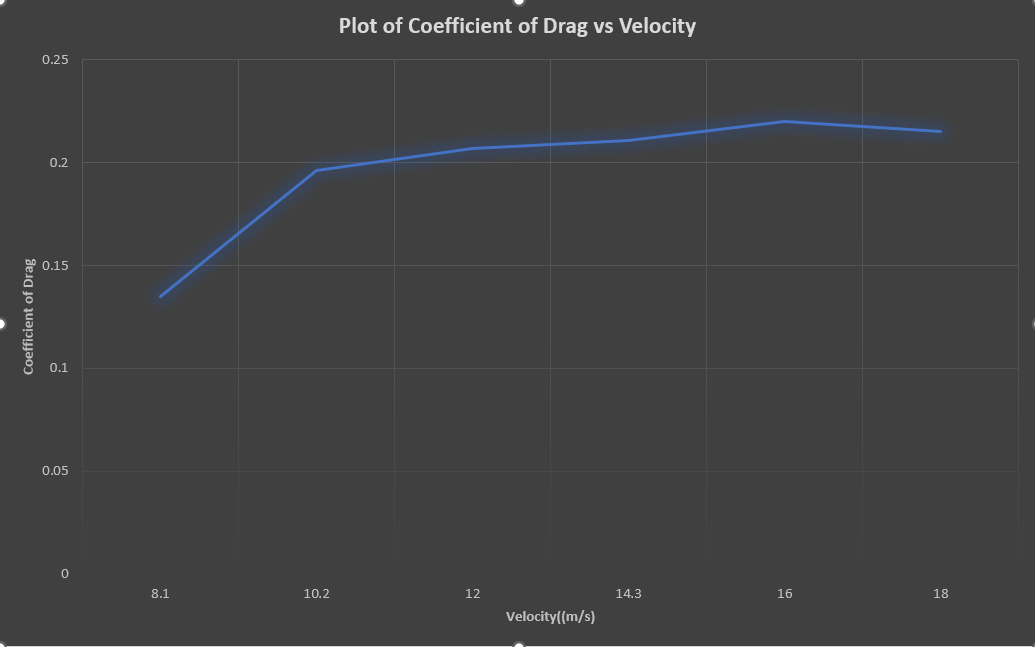
\includegraphics[scale=0.6]{exp5.4.png}
		}
	\end{center}
	\caption{Variation of theoretical and experimental $C_p$ with Angles}
\end{figure}

\newpage














\section{Calculations :}


\subsection{Calculation of Coefficient of Pressure :}
Coefficient of Pressure :
$$C_p = \frac{P - P_{\infty}}{\frac{\rho v^2}{2}} = 1 - 4 sin ^2{\theta}$$
For velocity 10.2 m/s , \\
Gauge pressure at $0^{\circ}$ = -0.3 mm of water = 2.94 = P-$P_{\infty}$\\
\vspace{2mm}
Experimental $C_p$ = $\frac{P - P_{\infty}}{\frac{\rho v^2}{2}}$ = $\frac{-0.3 \times 9.8}{(1/2)\times 1.293 \times 10.2^2} = -0.044 $



Theoretical $C_p =  1 - 4 sin ^2{\theta} = 1 $ (Putting $\theta = 0^{\circ}$ )\\


\subsection{Calculation of coefficient of Drag :}
 $\Rightarrow$ \textbf{Drag :}
\[ D = \sum_{i=1}^{10} (P-P_{\infty})r (cos\theta_i) \Delta\theta_i \] 
For velocity 10.2 m/s ,\\
$$ D = 1.24 N $$ \\
\textbf{Coefficient of Drag :}
$$ C_d = \frac{D}{(1/2)\rho v^2 S} = \frac{1.24}{(1/2)\times 1.293 \times 10.2^2 (2\pi \times 15 \times 10^{-3})} = 0.196
$$









\section{Sources of Error:}
\begin{itemize}
    \item Error due to instrumental defect.
    \item Error may occur in taking readings before flow becomes steady.
    \item Error due to environmental effect like temperature,pressure change.
    \item Error in measurement due to presence of zero error in parameters.
\end{itemize}



\section{Conclusion :}
\begin{itemize}
    \item Theoretical seperation point is found just before $120^{\circ}$ $(\approx 110 ^{\circ})$ but experimentally it is found between $140^{\circ}  and  160^{\circ}$ .
    \item Experimental variation of $C_p$ deflects a litle from thepretical variation of $C_p$ with angles.
    \item Drag first increases then remains almost constant on increasing flow velocity.
\end{itemize}


\end{document}